\section{Introduction}

Patient simulators are the cornerstone of clinical decision support solutions, providing a means to validate the efficacy of medical interventions in silico so cheaply that reinforcement learning algorithms can be used to develop protocols of clinical interventions automatically.
Unlike other machine learning applications, notably language modeling that can obtain a near-unlimited amount of data from the internet\footnote{See CommonCrawl \cite{commoncrawl} \url{commoncrawl.org}}, Healthcare suffers from an acute shortage of training data \cite{datashortage}.
As a result, many existing patient simulators are not trained on data from real patients, but instead rely upon expert knowledge \cite{towards}, leading to issues like \emph{confirmation bias} (the types of interventions currently favoured by clinical experts will work well in simulators developed by said experts irregardless of their real-world performance) and a high Sim2Real \cite{sim2real} gap.

In this work, we utilize a dataset of fetal ultrasound images to propose a novel data-driven patient simulator for decision support and automation in the field of obstetric ultrasonography \cite{obstetrics-sonography}.

The goal of this simulator is to accurately model the job of an ultrasound sonographer in the context of a patient undergoing a pregnancy in a way compatible with modern Reinforcement Learning methods \cite{rl-review}
to pave the way for autonomous or semi-autonomous ultrasound sonography \cite{autonomous-ultrasound-review}.
The job in question entails moving the ultrasound probe along the patient's body in order to acquire an image of the fetus that satisfies the guidelines for fetal-screening \cite{isoug-guidelines}, most importantly, the fact that the fetus' stomach and umbilical vein are on the image while their heart is not.

\newpage
\section{Methodology}

\paragraph{Dataset}

\begin{figure*}
    \centering
    \begin{subfigure}{.45\linewidth}
      \centering
      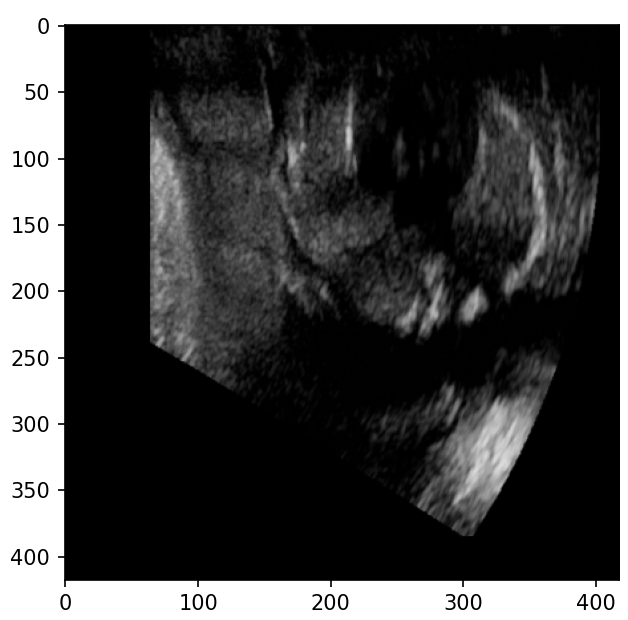
\includegraphics[width=.95\linewidth]{fetal_start.PNG}
      \caption{Starting point: the probe is located at the exact average of available positions. Heart, stomach and umbilical vein are unseen.}
      \label{fig:img-before}
    \end{subfigure}%
    \begin{subfigure}{.45\linewidth}
      \centering
      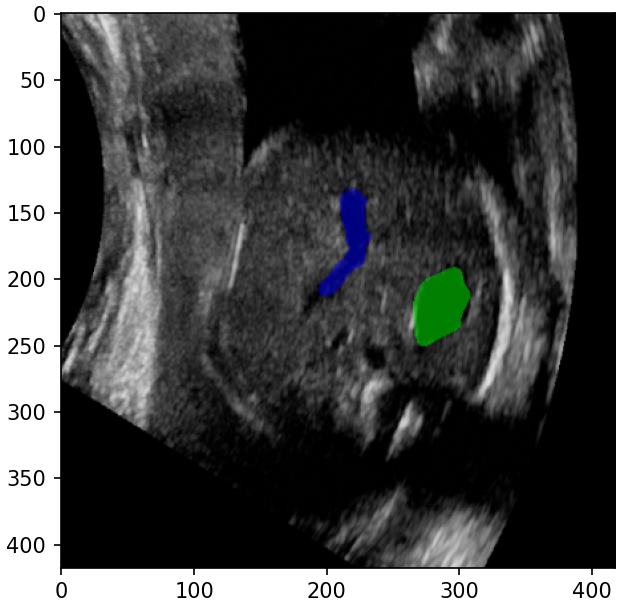
\includegraphics[width=.95\linewidth]{fetal_goal.PNG}
      \caption{Endpoint: stomach (green) and umbilical vein (blue) are present, heart is absent.}
      \label{fig:img-after}
    \end{subfigure}
    \caption{Two examples of the agent's observation at different positions of the probe}
    \label{fig:imgs}
\end{figure*}

The simulator is based on a dataset of 3D volumes representing fetal abdominal ultrasound scans (though be easily adapted to other medical imaging scenarios as long as a dataset of volumes and relevant organ annotations is available).
Each scan is a function defined over a cuboid $B$ of size $\langle x_\text{max},y_\text{max},z_\text{max} \rangle$ (in millimeters).
\begin{equation}
    I(x,y,z): B \rightarrow [0;1]
\end{equation}

Each scan is accompanied by three mask images $M_\text{heart}$, $M_\text{stomach}$ and $M_\text{uv}$ over the same domain, indicating which parts of the scan are considered to be the heart, the stomach and the umbilical vein respectively.

\begin{equation}
    M(x,y,z): B \rightarrow \{0,1\}
\end{equation}

\paragraph{Framework}

We adopt the industry-standard framework of {\em Episodic Partially Observable Markov Decision Process} \cite{kramerjdavidrPartiallyObservableMarkov1964, spaanPartiallyObservableMarkov2012}, implemented as OpenAI Gym \cite{gym} where every simulator is a 8-tuple of non-terminal state space $\mathcal{S}$, action space $\mathcal{A}$, observation space $\mathcal{O}$, stochastic observation model $\mathcal{O}, p_o(o | s, a)$, stochastic transition model $p_s(s_\text{next} | s_\text{prev}, a)$, stochastic reward model $p_r(r | s, a)$, initial state distribution $p_\text{init}(s)$ and episode termination model $p_\text{end}(s)$.

\paragraph{State}

The state, in this case, is the current position of the proble defined by 2 3-vectors, the position of the probe $s_\text{loc} \in \mathcal{S}_\text{loc}$ and its direction $s_\text{dir} \in R^{3}$.

The simulator has 2 modes for the space of possible locations $\mathcal{S}_\text{loc}$: \emph{free} and \emph{realistic} movement.
In \emph{free movement} mode, $\mathcal{S}_\text{loc} = B$, thus the agent can place the probe anywhere within the bounds of the image, even inside the patient.
In \emph{realistic movement} mode, $\mathcal{S}_\text{loc} \subset B$ representing the surface of the patient's body available to the agent.

\paragraph{Actions}

The action space $\mathcal{A} = R^{7}$, where any $a \in \mathcal{A}$ can be decomposed as

\begin{equation}
    a = (a_{x} , a_{y} , a_{z} , a_\text{roll} , a_\text{pitch} , a_\text{yaw}, a_\text{end})
\end{equation}

The first 3 components modify the $s_\text{loc}$, the next 3 modify $s_\text{dir}$ and, finally if $a_\text{end} > 0$, the episode terminates and the current image is considered final.
Note that in \emph{realistic movement} mode, blind application of $(a_{x} , a_{y} , a_{z})$ can lead to the probe being placed outside of the allowed domain of $\mathcal{S}_\text{loc}$.
In this case, a legal location will be chosen, in a manner that minimizes the distance between requested and real probe position:

\begin{equation}
    s_\text{loc} \leftarrow \min_{s \in \mathcal{S}_\text{loc}} \left\{ \lVert s - (s_\text{loc} + (a_{x} , a_{y} , a_{z})) \rVert \right\}
\end{equation}

\paragraph{Observations}

The observation is obtained by projecting $I(x,y,z)$ onto a plane defined by the current position of the probe $s_\text{loc}$ and its direction $s_\text{dir}$, simulating the image that the sonographer would see on their screen.
It is, theoretically, a function $I_\text{proj}(x_\text{proj}, y_\text{proj})$, however, since it is customary in POMDP framework for observations $o$ to be matrices, we replace it with a matrix of evaluations of $I_\text{proj}(x_\text{proj}, y_\text{proj})$ on an arbitrary (hyperparametrized) coordinate grid $\{(x_\text{proj}, y_\text{proj})\}$.

\paragraph{Rewards}

The quality of the image is defined in accordande with ISOUG guidelines \cite{isoug-guidelines} to be measured by the surface area of the heart, the stomach and the umbilical vein on the projection, normalized by the volume of these organs.

\begin{equation}
    Q(I_\text{proj}) = \frac{S_\text{stomach}(I_\text{proj})}{V_\text{stomach}(I)} + \frac{S_\text{heart}(I_\text{proj})}{V_\text{heart}(I)} + \frac{S_\text{uv}(I_\text{proj})}{V_\text{uv}(I)}
\end{equation}

The reward then is the diffence in quality between the current image and the one obtained at the previous iteration, so that probe movements that improve the image are rewarded positively and all rewards obtained during the episode sum up to the quality of the chosen image.

\newpage
\section{Related work}

Another simulator with a somewhat similar methodology is SonoRL \cite{sonorl}. The most important differences underlining the need for this simulator are:
\begin{itemize}
    \item SonoRL models ultrasonography of the spine (\emph{paramedian sagittal lamina view} \cite{spinal-guidelines}), while we focus on fetal screening.
    \item The reward function in SonoRL is a vector distance between the current position of the probe and the correct position. However, in reality, "correct" locations of the probe are numerous, comprising an equivalence class of solutions that satisfy the requirements in \cite{isoug-guidelines}.
    \item The implementation of SonoRL is not available to the wider community.
\end{itemize}

\newpage
\section{Future work}

One direction is to provide the observations in a low dimentional format.
At present, the neural network in charge of the agent is solving 2 separate tasks simultaneously: interpreting the image and making probe movement decisions based on it. Assigning this task to specialized components typically increases the agent's performance \cite{decoupling-rl}. Adding a feature extractor that will find relevant details in the image and replacing the image observation space with the space of these features would let the agent specialize purely in decision-making.

Besides, Healthcare automation raises specific concerns \cite{health-ai-explainability1,health-ai-explainability2} about the explainability of underlying models. 
As a way to make the agents more explainable, Programmatically Interpretable Reinforcement Learning \cite{pirl,neurogenetic} would be a logical extension of this work.
